%%%
%
% $Autor: Siddhanth Sharma, Nayan Chavan, Gargi Barve $
% $Date: 2024-10-31 11:15:45Z $
% $File: file.tex $
% $Version: 2 $
%
% Project: BA26-04 Time Series Forecasting CPI Germany
%
%%%

\chapter{Methodology: KDD}
\label{ch:kdd-methodology}

The methodological backbone of this project is the \textbf{Knowledge Discovery in Databases (KDD)} process \cite{Fayyad:1996}. This choice is appropriate because the CPI forecasting system is not limited to model fitting alone. The project begins with selecting an official public dataset, continues through preprocessing and transformation, applies statistical forecasting models, and extends further into evaluation, deployment, monitoring, and iterative reuse. A methodology that covers this full sequence is therefore more suitable than an ad hoc modeling description.

In the context of this project, the KDD process can be mapped to a development-and-deployment workflow. The \textbf{database and selection} steps correspond to choosing Germany's monthly CPI from the Destatis GENESIS database, specifically table 61111-0002. The \textbf{preprocessing} step is implemented in \texttt{Code/src/data\_loader.py}, where metadata rows are skipped, year values are forward-filled, months are parsed, missing CPI values are removed, and a strict monthly index is enforced. The \textbf{transformation} step appears in the exploratory workflow through differencing, ADF testing, decomposition, and autocorrelation analysis. The \textbf{data-mining} step is realized by fitting ARIMA, ETS, and SARIMA models in \texttt{Code/src/models.py} and \texttt{Code/src/modeling\_pipeline.py}. The \textbf{evaluation and verification} step compares the resulting forecasts with the holdout period by means of RMSE, MAE, and MAPE. After model training, the workflow moves into \textbf{deployment}: saved artifacts are reused in the Streamlit application for inference and result presentation, while \textbf{monitoring} captures the role of new monthly CPI releases and the feedback loop that can trigger renewed pipeline execution.

\begin{figure}[htbp]
    \centering
    \tikzstyle{mainblock} = [rectangle, rounded corners=2pt, minimum width=2.55cm, minimum height=1.15cm, text centered, align=center, draw=blue!60!black, fill=blue!18]
\tikzstyle{dbblock} = [mainblock, fill=red!18]
\tikzstyle{mineblock} = [mainblock, fill=green!22]
\tikzstyle{modelblock} = [mainblock, fill=yellow!22]
\tikzstyle{evalblock} = [mainblock, minimum width=3.0cm, minimum height=1.05cm, fill=blue!18]
\tikzstyle{flow} = [->, >=stealth, draw=blue!60!black]
\tikzstyle{lineflow} = [-, >=stealth, draw=blue!60!black]
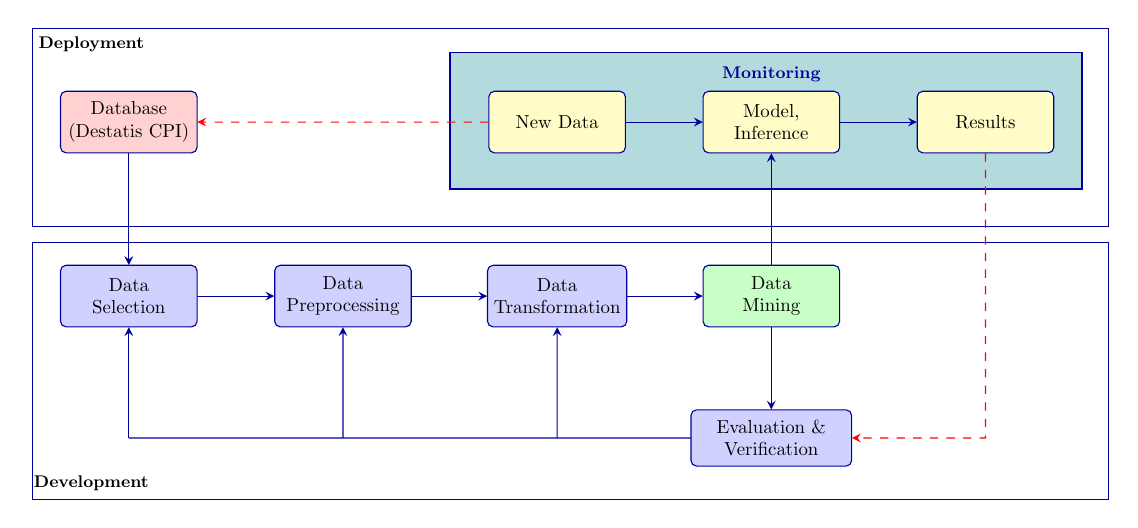
\begin{tikzpicture}[scale=0.68, every node/.style={transform shape}]
    \draw[draw=blue!60!black, line width=0.5pt] (-1.8,1.3) rectangle (18.3,5.0);
    \draw[draw=blue!60!black, line width=0.5pt] (-1.8,-3.8) rectangle (18.3,1.0);
    \fill[fill={rgb,255:red,138; green,198; blue,203}, fill opacity=0.65] (6.0,2.0) rectangle (17.8,4.55);
    \draw[draw=blue!60!black, line width=0.5pt] (6.0,2.0) rectangle (17.8,4.55);
    \node[font=\small\bfseries, text=blue!60!black] at (12.0,4.15) {Monitoring};

    \node (db) [dbblock] at (0,3.25) {Database\\(Destatis CPI)};
    \node (newdata) [modelblock] at (8.0,3.25) {New Data};
    \node (inference) [modelblock] at (12.0,3.25) {Model,\\Inference};
    \node (results) [modelblock] at (16.0,3.25) {Results};

    \node (sel) [mainblock] at (0,0) {Data\\Selection};
    \node (prep) [mainblock] at (4.0,0) {Data\\Preprocessing};
    \node (trans) [mainblock] at (8.0,0) {Data\\Transformation};
    \node (mine) [mineblock] at (12.0,0) {Data\\Mining};
    \node (eval) [evalblock] at (12.0,-2.65) {Evaluation \&\\Verification};

    \node[font=\small\bfseries] at (-0.7,-3.5) {Development};
    \node[font=\small\bfseries] at (-0.7,4.70) {Deployment};

    \draw [flow] (db.south) -- (sel.north);
    \draw [flow] (sel.east) -- (prep.west);
    \draw [flow] (prep.east) -- (trans.west);
    \draw [flow] (trans.east) -- (mine.west);

    \draw [flow] (mine.north) -- (inference.south);
    \draw [flow] (newdata.east) -- (inference.west);
    \draw [flow] (inference.east) -- (results.west);

    \draw [flow] (mine.south) -- (eval.north);
    \draw [lineflow] (eval.west) -- (0.0,-2.65);
    \draw [flow] (0.0,-2.65) -- (sel.south);
    \draw [flow] (4.0,-2.65) -- (4.0,-1.05) -- (prep.south);
    \draw [flow] (8.0,-2.65) -- (8.0,-1.05) -- (trans.south);

    \draw [flow, dashed, red] (results.south) -- (16.0,-2.65) -- (eval.east);
    \draw [flow, dashed, red] (newdata.west) -- (1.30,3.25) -- (db.east);
\end{tikzpicture}

    \caption{KDD-oriented machine-learning pipeline used in the CPI forecasting project. The lower layer captures the development workflow from data selection to evaluation and verification, while the upper layer represents deployment, result serving, new data intake, and monitoring-driven feedback.}
    \label{fig:kdd-ml-pipeline}
\end{figure}

\begin{table}[htbp]
    \centering
    \caption{Mapping of KDD stages to repository implementation. Source: own mapping based on the KDD process \cite{Fayyad:1996}.}
    \label{tab:kdd-mapping}
    \begin{tabular}{p{3cm}p{9.5cm}}
        \hline
        KDD stage & Repository realization \\
        \hline
        Database / Selection & Destatis CPI table 61111-0002 as the single official data source \\
        Preprocessing & \texttt{Code/src/data\_loader.py} \\
        Transformation & \texttt{Code/src/eda\_pipeline.py} and related diagnostics \\
        Data Mining & \texttt{Code/src/models.py} and \texttt{Code/src/modeling\_pipeline.py} \\
        Evaluation / Verification & Metrics, plots, exported CSV results, and holdout-based model comparison \\
        Deployment / Inference & \texttt{Code/app.py} together with serialized model artifacts in \texttt{Code/saved\_models/} \\
        Results & Interactive forecast plots, confidence intervals, and model metrics presented in the Streamlit interface \\
        Monitoring / New Data & Monthly CPI file replacement, pipeline reruns, and metric comparison as discussed in the monitoring chapter \\
        \hline
    \end{tabular}
\end{table}

This mapping is especially useful for a forecasting project because it makes clear that forecast quality depends on all earlier stages, but also that the workflow does not stop after model fitting. An incorrectly parsed month, a missing observation, or an inconsistent frequency would affect the final model comparison just as directly as a poor hyperparameter choice. At the same time, a deployment-oriented system must still account for inference, result communication, and the possibility that newly published CPI data will require renewed execution of the pipeline. The KDD framework therefore gives the report a coherent structure while also reflecting the actual software architecture of the repository.

\section{Justification for Using KDD}

The KDD process was chosen for this project because it provides a structured, data-centric approach that aligns well with the goal of extracting meaningful forecasts from historical CPI data. Its clear focus on data transformation and interpretation supports the creation of time-based features essential for accurate inflation forecasting. The following subsections explain why KDD is particularly suitable for this project.

\subsection{Data-Centric Nature Fits Time Series Projects}

KDD is fundamentally a data-driven methodology. Since time series forecasting relies on data structure, temporal dependencies, and trend patterns, the KDD framework helps navigate from raw statistical exports to forecast-ready data. In this project, the Destatis CPI table is not immediately usable for modeling: it contains metadata rows, textual month names, forward-filled years, and missing-value markers. The KDD preprocessing and transformation stages provide the natural place to document these cleaning steps, which would be lost if the report jumped directly to model equations.

\subsection{Structured Transformation Emphasis}

The KDD process places special focus on the transformation phase, where new features and analytical structures are created. In this project, transformation includes differencing for stationarity assessment, seasonal decomposition for pattern identification, and autocorrelation analysis for model order selection. These transformations are central to time series forecasting, especially when using classical models that do not natively understand date-time context. Without an explicit transformation stage, the justification for model hyperparameters would be weaker.

\subsection{Iterative, Yet Linear Flow Works Well}

KDD follows a linear progression from selection to interpretation, making it easier to implement and track steps in a controlled academic setting. Each step in this project prepares the data further and builds toward accurate and interpretable forecasting. The linear structure also leads cleanly into the final dashboard output, because the deployment layer consumes artifacts created at each preceding stage. This traceability is valuable for both grading and reproducibility.

\subsection{Interpretability of Results}

The final KDD stage, interpretation, fits perfectly with the project's use of forecast plots, interactive dashboard elements, and business-relevant metric comparisons. KDD supports turning complex numerical output into knowledge that non-technical stakeholders can understand. In this project, the Streamlit dashboard serves exactly this purpose: it makes the forecasting results accessible without requiring the user to read Python code or statistical tables.

\subsection{Ideal for Academic and Research Projects}

Because KDD is academically recognized and well documented, it provides a research-friendly structure that allows each phase to be clearly defined and referenced. This strengthens the project's credibility, especially for evaluation and grading, because the report can point to a known methodology rather than presenting an ad hoc workflow. The KDD framework also makes it easier for other researchers to reproduce the work, because the stage boundaries are explicit and the repository files map cleanly to each stage.

\subsection{Final Justification Statement}

The KDD process was chosen for this project due to its strong alignment with data-driven forecasting, its clear structure from raw data to knowledge discovery, and its focus on transformation and interpretability. By applying KDD, the project was able to systematically clean, enhance, model, and communicate CPI patterns and predictions through a well-organized workflow and interactive dashboard.

\section{Methodology Boundary}

The methodology also has a practical boundary. It structures the analytical and technical pipeline, but it does not by itself provide complete guidance for project organization, collaboration, or production infrastructure. For this reason, the later report chapters complement the KDD framework with development, deployment, validation, and monitoring considerations specific to the CPI forecasting application.
